\chapter{Collaborative Gate Counting}
\label{cha:gate-counting}

In this chapter, we tackle one of the most common forms of urban
sensing: counting unique visitors across multiple gate counters to
measure the flow of people across the urban setting. 

\section {Motivation and System Model}
\label{sec:motivation}

Bluetooth scanners register the Bluetooth addresses, 48-bit MAC, of
the devices that have been sighted. The Bluetooth device address is a
48-bit MAC format address that uniquely identifies each Bluetooth
device. Some devices are able to switch between multiple Bluetooth
addresses, but for most cases this will be a reliable and permanent
unique identifier for sighted devices and by extension to the
respective owners. A single scan of nearby devices is not in itself
much of a problem. However, a systematic registration of Bluetooth
sightings, especially when done at multiple locations, has the
potential to become a large scale tracking system given the personal
nature of most Bluetooth devices. Relatively simple processes can be
put in place to detect the presence, movements and patterns of
individuals. Concerning anonymity, the absence of a public record
mapping Bluetooth addresses to specific individuals is nothing but a
fragile barrier. To track a specific individual, it would suffice to
intersect the Bluetooth addresses from some of the places she has
visited. Eventually, all that would have been left is a single
Bluetooth address which could then be used to easily track that person
from that moment on. To prevent cases like this, a privacy preserving
approach should avoid permanent storage and dissemination of Bluetooth
addresses or of any other information that could uniquely identify an
individual.

Our Gate Counting scenario assumes the existence of a large set
of heterogeneous and autonomous Bluetooth nodes. We use the terms
\emph{node} and \emph{scanner} interchangeably throughout this document.
Conceptually, a gate is a virtual line across a street, and gate
counting is the process of counting the number of people crossing that
line. Each Bluetooth node is modeled as a gate counter that counts the
number of unique Bluetooth addresses observed during a certain period.
The use of Bluetooth as an enabling technology to establish the flows
of people it not a new concept. There are several examples, be it
within a city~\cite{Oneill:2006vq}, outdoor
festival~\cite{versichele2012use} or shopping mall
~\cite{millonig2008shadowing}.

A Bluetooth-based gate counter does not really count all the persons
passing-by, but only those who are carrying discoverable Bluetooth
devices. Still, this is enough to make a reasonable correlation, using
baseline data, to estimate the overall traffic. A gate counter should
recognize subsequent sightings of the same entity. In a gate counting
scenario, repeated sightings of the same device can be very common,
not only because people can be passing-by multiple times, but also
because of persistent devices. Instead of scanning through a line,
Bluetooth discovery is actually performed in an area and thus any
device in that area, possibly in nearby buildings, would be repeatedly
discovered. Results from empirical studies with known static and
transient devices suggest that a transient device typically appears
for up to 90 seconds while it crosses a gate \cite{Oneill:2006vq}. A
proper gate counting process would thus needs to account for this and
filter persistent devices.

A gate counter should also be able to answer questions like ``how many
different people were seen in a given gate in the last 24 hours?'' or
``what was the number of visitors of an amusement park during visitors
peak hours?''. To comply with this requirement, gate counters should
be able to distinguish its readings over time.

The main challenge, however, is how to enable collaborative counting
between multiple independent gate counters, while providing
appropriate privacy guarantees as well as low communication costs. To
be able to count unique entities, we need to identify multiple counts
of the same entity at different nodes, to make sure that the same
device sighted at two different gates will be counted only once.
Imagine, for example, a city festival with multiple gate counters
operating at various locations to count the number of visitors to the
festival. The simple sum of individual gate counts would clearly
overestimate the number of people since many of them would be spotted
at multiple gates. We thus need some technique that works across
multiple gate counters and is able to provide an aggregate count of
the unique device addresses that have been spotted in the entire set
of gate counters. Comparing the plain addresses observed at different
gates would immediately solve this problem, but as we have seen, it is
not suitable for privacy preservation.

\subsection{Objectives}
\label{sec:objectives}
 
In this chapter, we explore the use of stochastic summarizing
techniques as a privacy preserving approach to enable Bluetooth-based
gate counting of unique entities across multiple nodes. The objective
is to assess the extent to which these techniques are able to address the
specific requirements of this distributed gate counting model and
inform the design of large scale Bluetooth sensing systems.

Having identified the sensing requirements for this scenario we have
established a number of key criteria for assessing the various
alternatives. Using those criteria, we have conducted an
experimental study in which we compared how multiple types of
stochastic summarizing techniques would behave across multiple
variants of our gate counting scenario. The results provide a strong
foundation for the development of these large scale Bluetooth sensing
infrastructures, identifying major trade-offs and the implications of
key factors such as cardinality and support for merge operations.

% \section{Probabilistic counters for privacy-enhanced gate counting}
% \label{sec:techniques}
% % A common strategy in privacy-enhancing techniques is to reduce the data
% % collected to what is absolutely needed for a particular purpose. In this gate
% % counting scenario, we need to count devices and the ability to check if a
% % particular device has already been counted before. Moreover, we need to be able
% % to do this across a set of autonomous nodes. This means that we are not
% % interested in information about the number or duration of sessions that each
% % device generates at each gate.
% %we may want to know on which gate set a particular device has been seen, we do
% %not need to know the specific sequence through which the device has been seen at
% %those locations. 

% Probabilistic counters provide an interesting solution to this problem. They are
% flexible enough for estimating the overall number of unique sightings with some
% controllable accuracy, without ever keeping the plain Bluetooth addresses.


\section{Criteria}
\label{sec:Criteria}

This section tests some of the techniques mentioned in Section
\ref{sec:algorithms_and_data_structures}, namely LogLog Sketches
\cite{Durand:2003tc}, HyperLogLog Sketches \cite{Fusy:2007um}, LC
Sketches \cite{Whang:1990uh}, RIA-LC Sketches, 
\cite{Fan:2008wl,YaoChungFanArbeeLPChen:2010to}, RIA-DC Sketches
\cite{YaoChungFanArbeeLPChen:2010to}, Bloom Filters~\cite{Bloom1970}
and Scalable Bloom Filters~\cite{Almeida2007}. 

These techniques where picked because they provide an interesting
solution to this gate counting problem. Probabilistic counters are
flexible enough for estimating the overall number of unique sightings
with some controllable accuracy, without ever keeping the plain
Bluetooth addresses.

The requirements identified in section \ref{sec:motivation} boil down
to three important criteria: \textbf{accuracy}, \textbf{size} and
\textbf{aggregation}. These criteria were used in the evaluation the
proposed techniques.

%In the rest of this section we talk about the
%remaining criteria as well as of their respective requirements and analyze
%each technique regarding the aforementioned criteria.

% Processing power SHA1 - Energy Comparison of AES and SHA-1 for Ubiquitous
% Computing

\subsubsection{Accuracy} 
\label{sec:accuracy} 

With this criterion we want to evaluate the accuracy of the
techniques, their ability to count multiple sightings of the same
device only once, and the quality of their estimators. To do so, we
stipulated the maximum standard error for each technique. In this case
after setting it to  $5\%$, we measured for all % desvio padrão
techniques the relative error (root mean square error) for a range of
cardinalities, whose average of 100 runs is shown in
Fig~\ref{fig:accuracy}.

\subsubsection{Size}
\label{sec:size}
The size of the techniques is an important factor. The less space the
technique requires, the lower will be both the costs of communication
between BT scanners and their memory requirements.

Regarding this criterion, we have 2 fundamentally different
types of techniques: dynamic techniques which consist of Scalable Bloom
Filters and static techniques comprising the rest. Static
size techniques are techniques whose size is set at the time of creation and
cannot be changed afterwards. This means that we must know the maximum
number of unique devices to count before hand, or at least, we must be able
to assume an upper bound for that number. Dynamic techniques on the other
hand don't have this drawback because they can adjust to withstand
arbitrarily large cardinalities. In practical terms this means that for
static size techniques, once we create an instance with a certain capacity
it is not possible to change that capacity afterwards, while for dynamic
techniques there is no such constraint.

To further help us in our analysis, we can look at Figures
\ref{fig:bits_element} and \ref{fig:size}. Figure
\ref{fig:bits_element} depicts the number of bits per unique element
that each technique requires along a range of cardinalities. Figure
\ref{fig:size} shows the total size spent by each technique to store a
given number of distinct elements.

\subsubsection{Aggregation}
\label{sec:mergeAbility}

The ability to merge counts is crucial for scenarios with multiple
gates. It is a key ingredient for obtaining the \emph{aggregate
 number} of individuals in a set of gates. The merge operation
(Figure \ref{fig:merge}) consists in either a bitwise OR operation
(Bloom Filters, Linear Counting, RIA-DC and RIA-LC sketches) or in a
\emph{max} operation (HyperLogLog and LogLog sketches) of structures
that make each gate's counter. In order to merge several gate
counters, there are 2 conditions that must be met: all counters must
be instances of the same technique and every instance must have the
same parameters and capacity (equally sized bit arrays). Meeting these
conditions ensures that the same unique device will mark the same
positions in the several gate counters it crosses. Therefore after
merging the counters, it is possible to obtain the aggregate number of
unique elements without counting the same device repeatedly (Figure
\ref{fig:gate_counter_aggregation}).

\begin{figure}[htb]
\subfigure[\emph{max} Merge- used by LogLog and HyperLogLog Sketches]{
\label{fig:merge_hll}  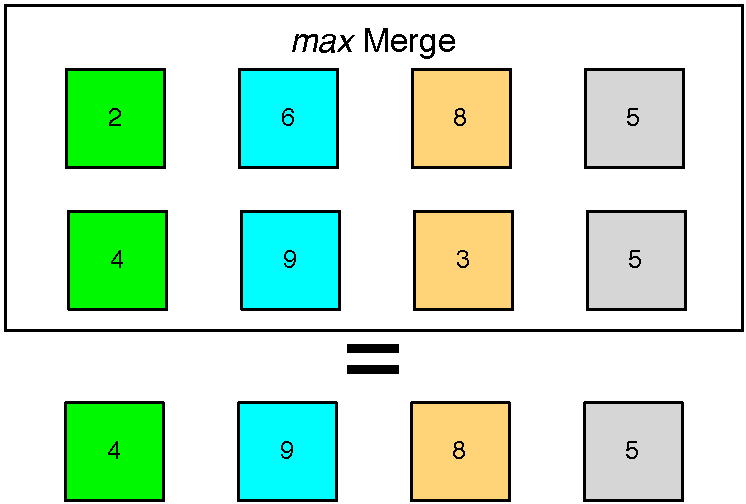
\includegraphics[scale=0.50]{images/merge_max.pdf}
}
\subfigure[Bitwise OR Merge - used by Bloom Filters, RIA-LC, RIA-DC and
LC Sketches]{
 \label{fig:size}  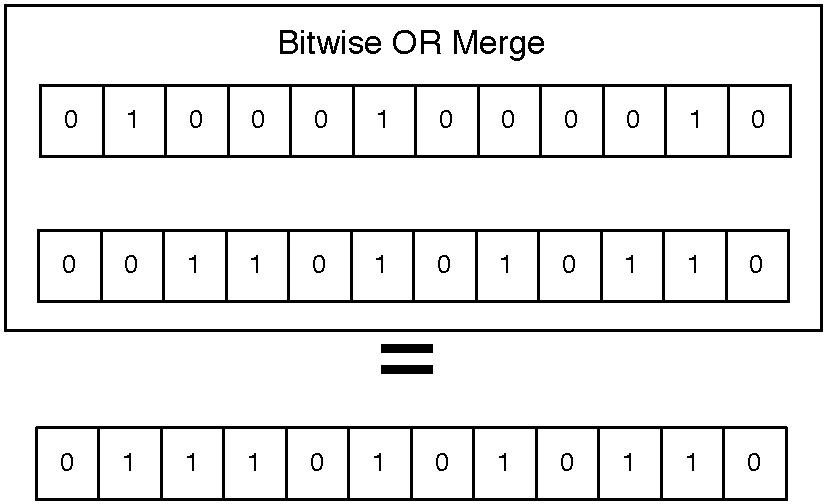
\includegraphics[scale=0.50]{images/merge_or.pdf}
}
\caption{Different Merge Approaches}
\label{fig:merge}
\end{figure}

\begin{figure}[htb]
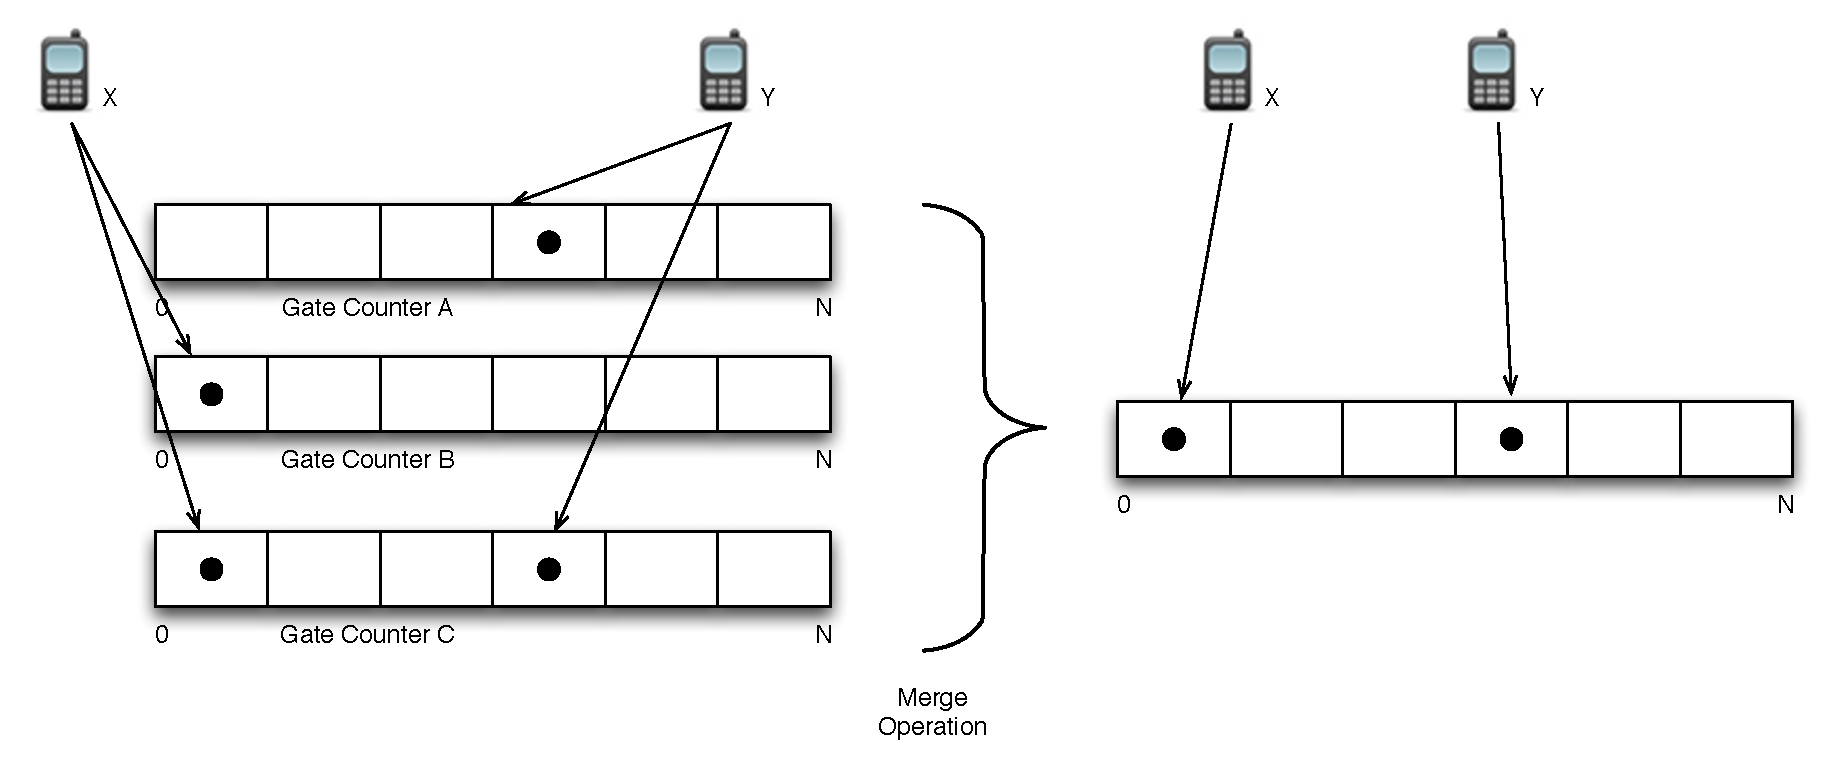
\includegraphics[width=\textwidth]{images/merge.pdf} 
\caption{Gate Counter Aggregation - repeated devices appear only once } 
\label{fig:gate_counter_aggregation} 
\end{figure}

With the exception of Scalable Bloom Filters and RIA-DC sketches, all
the techniques presented here have the ability to merge, and therefore
will not count the same device more than once in aggregate
counts. Scalable Bloom Filters lack the ability to merge because their
size varies dynamically with the number of unique elements, therefore
we cannot guarantee that the same unique device will set the same
positions for different filters. RIA-DC sketches might not provide
accurate aggregate results since the estimator considers there is no
overlap of elements between the different counters.

Aggregation is also important as a mean for answering time related
questions like ``how many different people were seen in a given gate
in the last 24 hours ?'' or ``what was the number of visitors of an
amusement park during visitors peak hours?''. To answer these types of
questions, it must be possible to distinguish/segment counter readings
over time. This can by accomplished by sensor nodes periodically
making a copy of their counters followed by a reset. Those copies will
keep the information about the unique devices sighted during a certain
time period. For example, considering that the rate at which counters
are saved and reset is 1 hour, the former question could be answered
by merging the 24 last saved counters. To answer the latter, we would
need to merge the copies made during peak hours at the various nodes
in the park.

To save some space, we can use different time granularities. For
instance, we can merge all unique counters saved during a day and
obtain the aggregate count for the day, merge the counters from the
last 7 days and get the aggregate count for the week, and so forth. We
just need to keep in mind that because of the merge restrictions, the
size of the counter that stores the unique number of devices sighted
during an hour has to big enough to fit the number or unique devices
seen during the entire week.

As we can see both \emph{time segmentation} and \emph{aggregate counting}
are in fact variations of the same problem, which can only be solved with
techniques that support merging. 

\begin{figure}[htb]
%\centering
\subfigure[Upper bound $10^2$]{
\label{fig:accuracy0_1k}  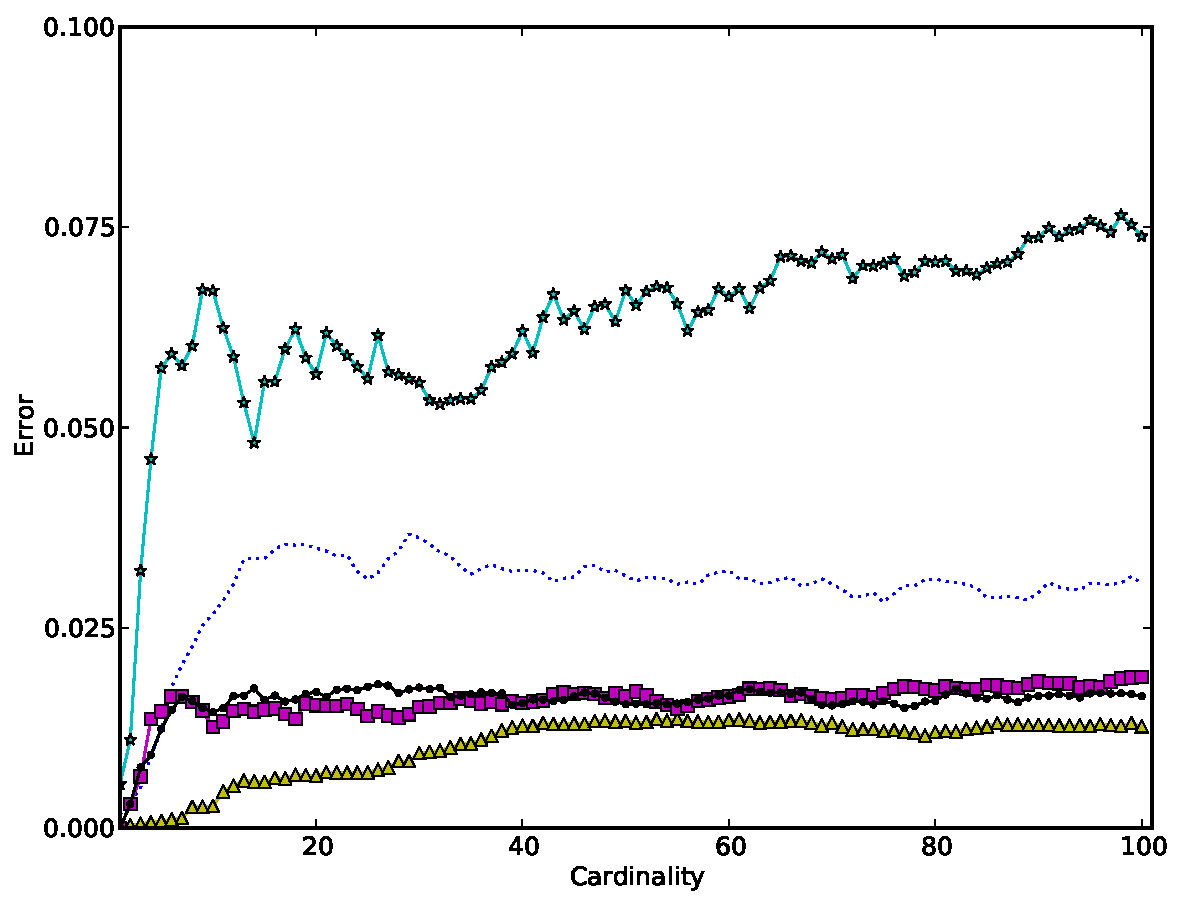
\includegraphics[scale=0.35]{images/0_1k100xAcc.pdf}
}
\subfigure[Upper bound $10^3$]{
 \label{fig:accuracy1k}  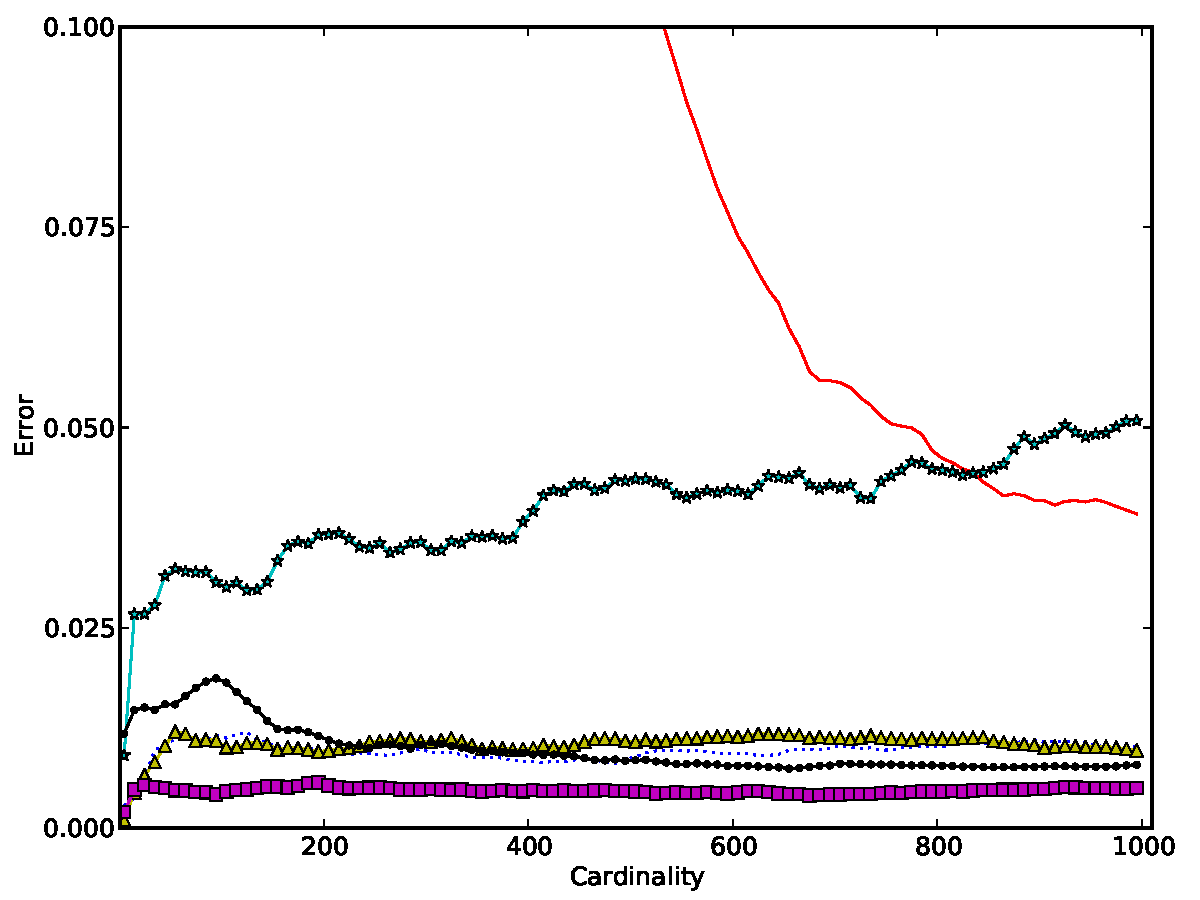
\includegraphics[scale=0.35]{images/1k100xAcc.pdf}
}
\subfigure[Upper bound $10^4$]{
  \label{fig:accuracy10k} 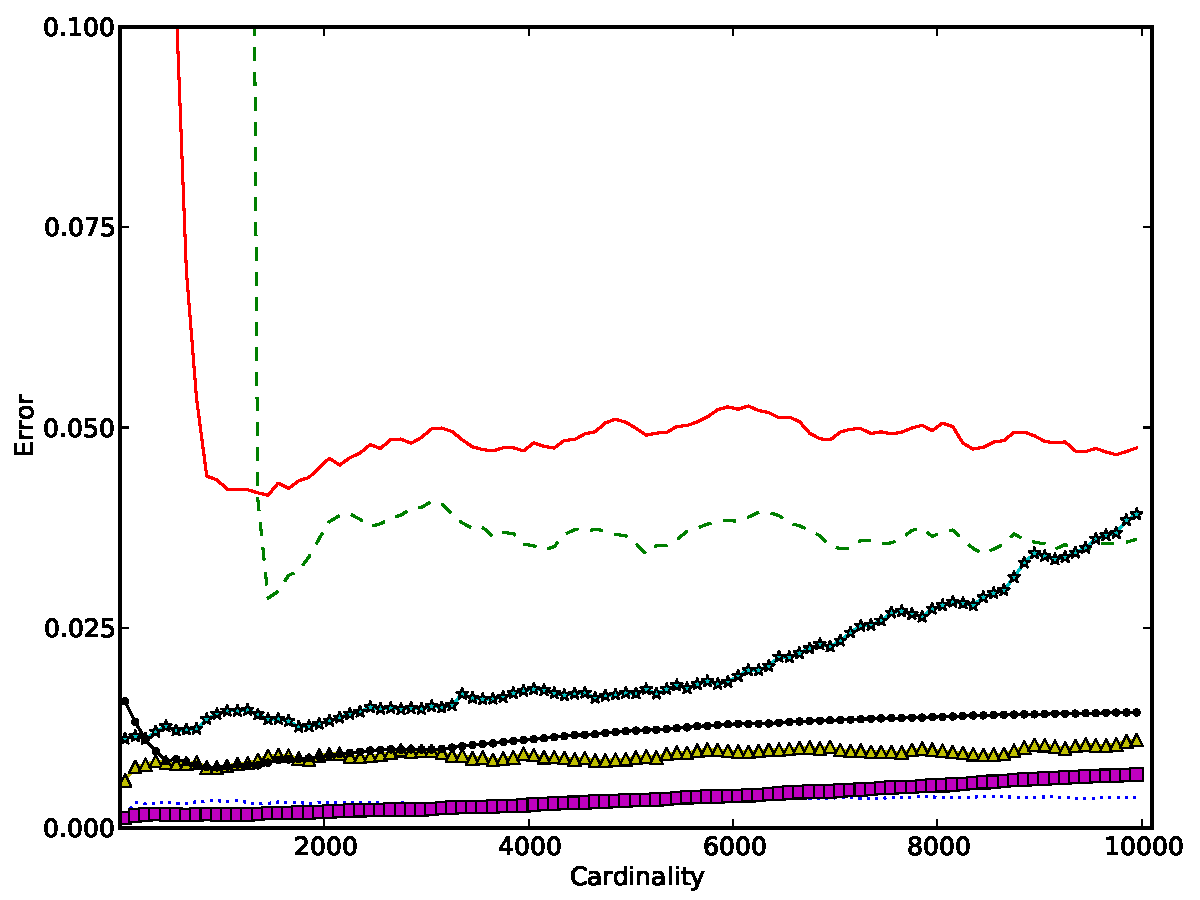
\includegraphics[scale=0.35]{images/10k100xAcc.pdf}
}
\subfigure[Upper bound $10^5$]{
  \label{fig:accuracy100k} 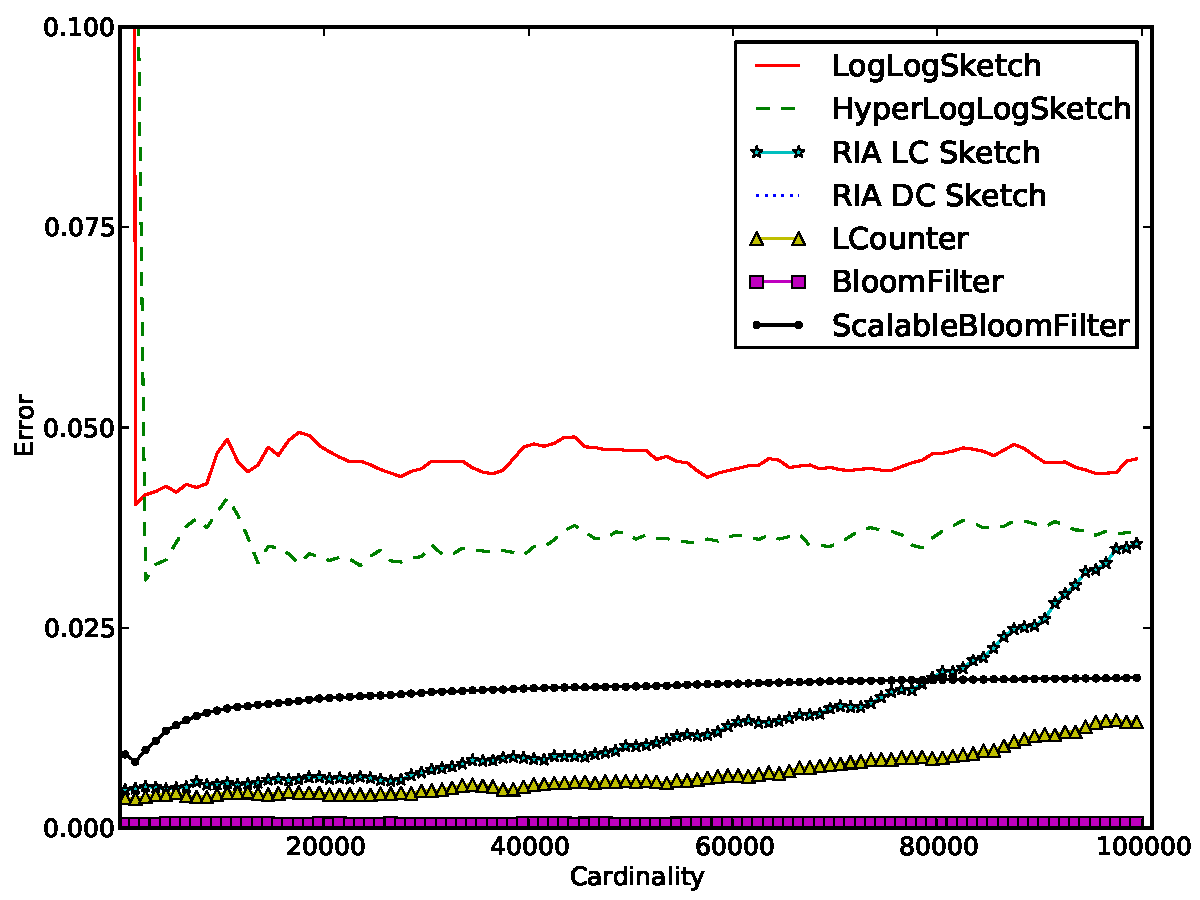
\includegraphics[scale=0.35]{images/100k100xAcc.pdf}
}

\caption{Relative error of the several techniques using various upper
  bounds. Average of 100 runs.} 
\label{fig:accuracy}
\end{figure}
   
\begin{figure}[htb]
%\centering
\subfigure[Number of bits per element used by each technique at different cardinalities]{
\label{fig:bits_element}  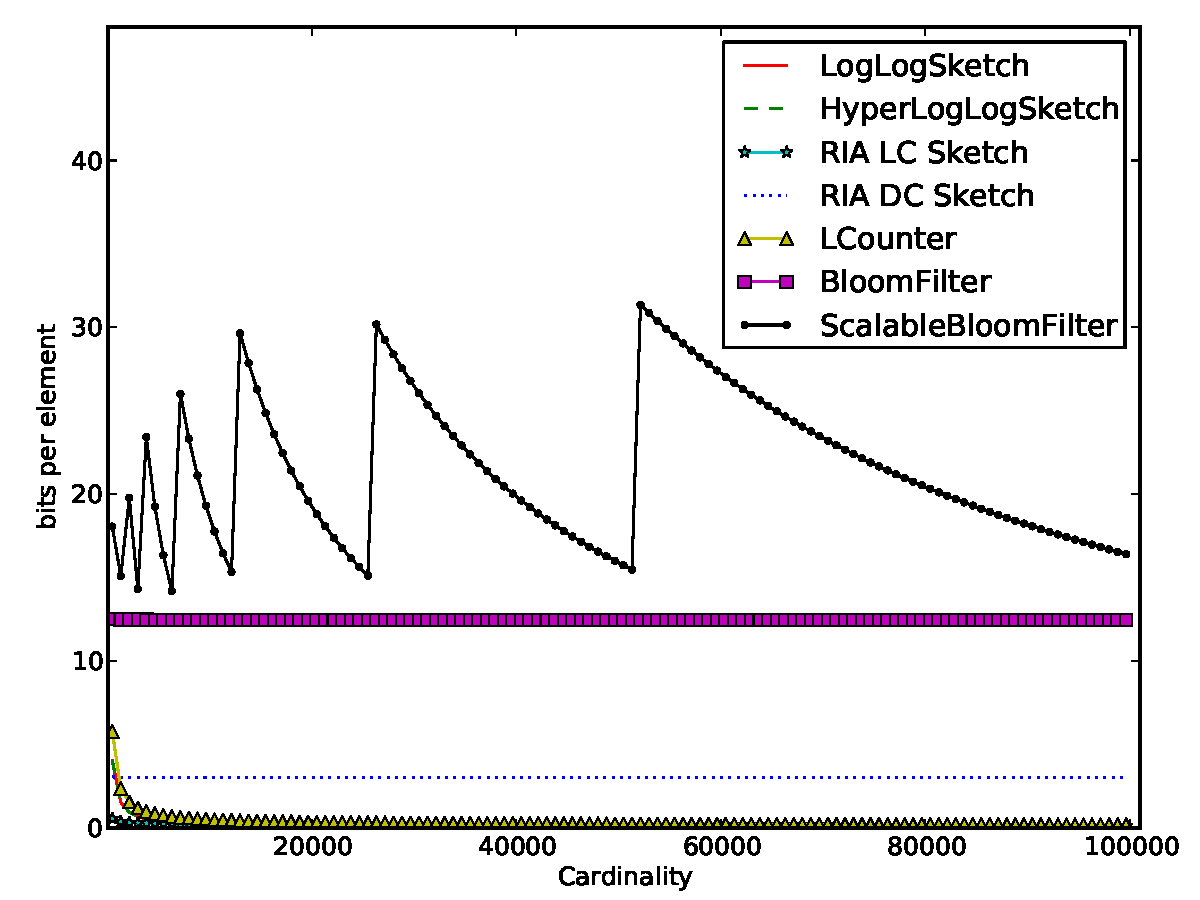
\includegraphics[scale=0.35]{images/bits_per_element_100k.pdf}
}
\subfigure[Size of the several techniques for different cardinalities]{
 \label{fig:size}  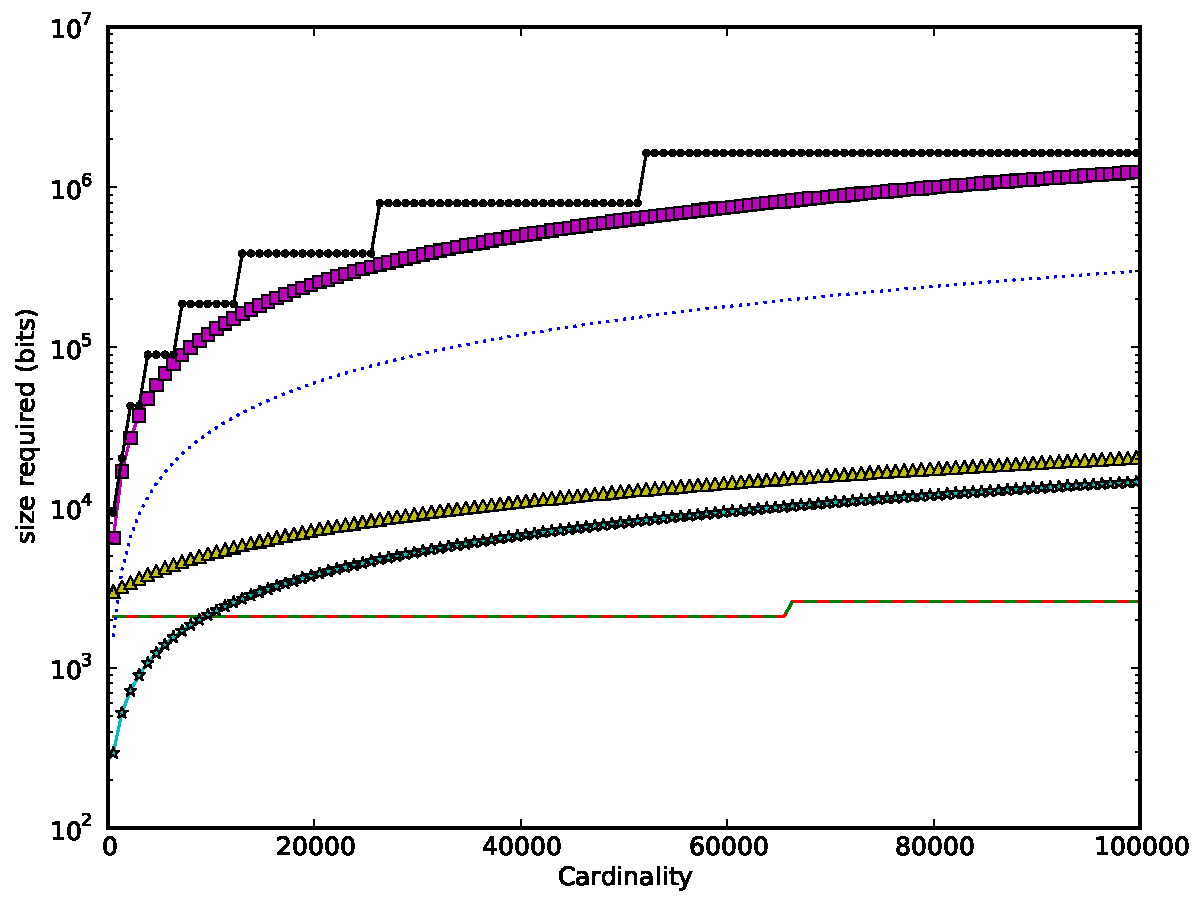
\includegraphics[scale=0.35]{images/size_100k.pdf}
}
\label{fig:size_benchmark}
\caption{Size benchmarks}
\end{figure}

\section{Evaluation}
\label{sec:evaluation}
Using the results from our benchmark\footnote{Our Benchmark was built
  in Python, including the implementation of the several algorithms,
  with the exception of Bloom Filters where we used Jay Baird's
  implementation.} shown in figures \ref{fig:accuracy} and
\ref{fig:size_benchmark} and having explained the
different criteria we can now analyze each one of the techniques.

\subsubsection{Standard and Scalable Bloom Filters} 
Both techniques provide a good accuracy for all the cardinalities
tested, never surpassing the stipulated relative error. Figure
\ref{fig:accuracy} confirms both these facts. However, looking at
Figure \ref{fig:size_benchmark} we can confirm that in regard to
space, they are the most expensive techniques of all. This extra cost
in terms of space stems from their query membership ability. Figure
\ref{fig:size_benchmark} also highlights the incremental nature of
Scalable Bloom Filters. Each time the filter gets full, a new Bloom
Filter is created, increasing the size of the technique. This explains
the seemingly strange behavior of the technique. Both these techniques
are also the most computationally expensive of all in terms of
insertion complexity.

\subsubsection{LogLog and HyperLogLog Sketches} 
As depicted by Figures \ref{fig:accuracy0_1k} and
\ref{fig:accuracy1k}, these techniques have very low accuracy for
small cardinalities ($\lesssim 1800$). Apart from this issue, they are
the best suited techniques for large cardinalities due to their
logarithmic growth in size. As shown in Figure \ref{fig:size}, for
numbers of distinct elements above 10000, these are the most efficient
techniques in terms of space. Between the two, HyperLogLog sketches have
the advantage of being more accurate and of having a smaller
variance. Regarding insertion complexity, these techniques are less
expensive than Bloom Filters, but more expensive than the LC Sketches
based ones.

\subsubsection{LC Sketches, RIA-LC Sketches and RIA-DC Sketches} 
Spending only a little more memory than LogLog Sketches, LC Sketches
do not suffer from poor accuracy in smaller cardinalities, they have
good all around good accuracy just like Bloom Filters. LC Sketches are
a good all around technique. Being based on Linear Counting Sketches,
it is no surprise that RIA-DC and RIA-LC Sketches also have good
accuracy results. Furthermore and like their ancestor, they also
achieve good results in the bits per element ratio. These techniques
are also the ones with the smallest complexity in
terms of element insertion. \\

Taking into account all that has been said, there are a few
conclusions to be drawn. For scenarios where we cannot make
assumptions on the maximum number of elements to count, we have to use
Scalable Bloom Filters. For scenarios where there is a big discrepancy
between the cardinalities of different counters and where the
existence of repeated elements outside each counter can be neglected,
RIA-DC Sketches are probably the best choice. For scenarios with very
large cardinalities HyperLogLog Sketches are probably the correct
choice since they are the most space efficient technique.  Considering
the expected most common scenarios, where we need accurate aggregate
counts and where there is the possibility of counters with low
cardinalities, the choice falls either within Linear Counting Sketches
or RIA-LC Sketches. We prefer the latter since it is a slightly
simplified version of the former.

As a final remark, we should emphasize the fact that all the
techniques discussed in this chapter are more efficient in terms of
space than storing each unique device 48 bit MAC address (check
Fig.\ref{fig:bits_element}).

\section{Synopsis}
\label{sec:conclusion}
Bluetooth devices are pervasive in most societies and the number of unique
Bluetooth sightings is an adequate proxy for the number of actual individuals
present. The trivial approach of collecting and counting the set of detected
Bluetooth MAC addresses is not adequate, in most settings, both in terms of
privacy concerns, system scalability and adequacy to devices with limited
memory.  

In this chapter we described and benchmarked a set of stochastic summarizing
techniques that can be applied to the gate counting problem. By using these
techniques our approach ensures the privacy of the users since Gate Counters
don't store any extra raw information, i.e, the raw information that
they keep at any given moment is also present in the Bluetooth network. 
  
Furthermore, the analysis of these techniques and their trade-offs
should help to determine the most adequate solutions for a specific
gate counting scenario. % We also hope to have motivated the community
% to the relevant role of stochastic counting techniques in privacy
% preserving gate counting.

%%% Local Variables: 
%%% mode: latex
%%% TeX-master: "../thesis"
%%% End: 
